% !TEX root = ../../../main.tex
% 来源：中学数学实验教材·第三册（高中数学）
% 章节：任意角的三角函数 / 任意角的三角函数
% 原始文件：6.tex，行 714-725
% 类型：tikz
% ---
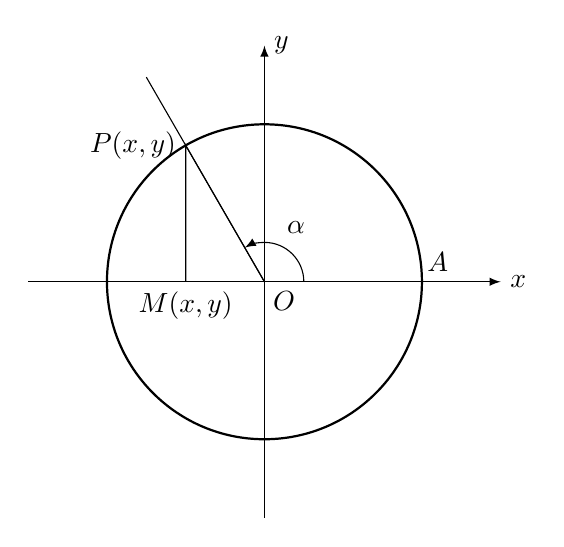
\begin{tikzpicture}[>=latex]
    \draw[->] (-3,0)--(3,0)node[right]{$x$};
    \draw[->] (0,-3)--(0,3)node[right]{$y$};
\draw[thick] (0,0) circle(2);
\draw (0,0)--(120:3);
\draw (0,0)--(120:2)node[left]{$P(x,y)$}--(-1,0)node[below]{$M(x,y)$};
   
\node at (2.2,0)[above]{$A$};   
\node at (.25,-.25){$O$};
\draw[->] (.5,0) arc (0:120:.5);
\node at (60:.8){$\alpha$};
\end{tikzpicture}
